\chapter{Konzept zur automatisierten Schmerzbewertung anhand akustischer Signale}
\label{sec:concept}

%Ergänenzen!
In Kapitel \ref{sec:medicalFoundations} wurde vorgestellt, wie die Schmerzdiagnostik bei Neugeborenen im medizinischen Alltag mit Hilfe multimodaler Schmerz-Scales durchgeführt wird. Das Ziel ist nun der Entwurf eines Konzeptes für ein System, das die Schmerzdiagnostik nach diesem Vorbild auf Basis akustischer Signale automatisiert und kontinuierlich vornimmt. In diesem Kapitel wird ein Überblick über das entworfene Konzept gegeben. Dazu wird in Kapitel \ref{sec:system_literature} zunächst ein Überblick über Veröffentlichungen mit ähnlichen Zielstellungen gegeben.

\section{Literaturüberblick}
\label{sec:system_literature}

Ein großer Teil der Veröffentlichungen, die sich in das Feld der Analyse von Audioaufnahmen Neugeborener einordnen lassen, stellen Methoden zur Klassifizierung einzelner Schreieinheiten vor, entweder bezüglich der Weinursache (Hunger, Angst, Schmerz, ... ) oder zur Diagnose bestimmter Krankheiten. Diese Methoden sind in den meisten Fällen nicht für eine kontinuierliche Analyse vorgesehen, sondern haben das Ziel, die Eignung bestimmter Features oder Klassifizierungsalgorithmen für die jeweiligen Klassifizierung zu erforschen. Beispiele für solche Veröffentlichungen sind die von Abdulaziz et al. \cite{class_abdulaziz} oder Fuhr et al. \cite{comparisonOfLearning}.

Várallyay stellte in seiner Dissertation \glqq Analysis of the Infant Cry with Objective Methods\grqq{} \cite{cry_thesis} Methoden zur automatisierten Analyse kindlicher Lautäußerungen vor. Das primäre Ziel der Dissertation war die Erforschung der Unterschiede zwischen den Lautäußerungen gesunder und tauber Neugeborener. Die Algorithmen zur automatisierten Analyse der Audiosignale waren ein \glqq Nebenprodukt\grqq{} zur schnelleren Datenauswertung. Die Auswertung musste nicht kontinuierlich erfolgen. In der vorgestellten Verarbeitungs-Pipeline wurde das Eingangssignal in Zeitfenster weniger Millisekunden zerlegt und jedes Fenster nach Entscheidungsregeln als \emph{stimmhaft} oder \emph{nicht stimmhaft} markiert. Die stimmhaften Signalfenster wurden zu \emph{Segmenten} zusammengefasst (welche in Kapitel \ref{sec:acousticModel} als Schreieinheiten bezeichnet werden). Auf Basis der Segmente wurden Auswertungen bezüglich des Zeitbereiches (Durchschnittliche Segmentlänge, Pausenlängen etc.), des Frequenzbereiches (Grund-Frequenz, Formanten-Frequenzen etc.) und des Melodieverlaufes vorgenommen. Analysiert wurden Audioaufnahmen von Babys mit einer Länge von 10 bis \SI{100}{\second}. Auf Basis der Auswertungsergebnisse stellte Varallyay die wichtigsten Unterscheidungsmerkmale zwischen tauben und gesunden Babys fest. In der Dissertation \cite{cry_thesis} wird ein Überblick über das Vorgehen und die Ergebnisse gegeben. Die Verarbeitungsschritte wurden detaillierter in einzelnen Veröffentlichungen beschrieben, wobei der Autor dieser Arbeit nur den Zugriff auf einige dieser Veröffentlichungen erhalten konnte.

Cohen et al. haben 2012 in der Veröffentlichung \glqq Infant Cry Analysis and Detection\grqq{} \cite{cohenCry}  ein System zur Analyse der akustischen Signale von Neugeborenen vorgestellt. Dieses System klassifizierte die Audiosignale in eine der drei Klassen \emph{Cry, No Cry} und \emph{No Activity}. Die Klasse \emph{Cry} bezeichnet Lautäußerungen, die eine potentiell Gefahr für das Baby anzeigen, wie z.B. wie Schmerz oder Hunger. Die Klasse \emph{No Cry} bedeutete, dass das Baby zwar Laute von sich gibt, diese aber keine potentielle Gefahr anzeigen. Die Klasse \emph{No Activity} bezeichnete keinerlei Lautäußerung. Die Verarbeitungs-Pipeline wurde detailliert vorgestellt und ist für die kontinuierliche Verarbeitung mit einer gewissen Verzögerungszeit spezialisiert. Das Signal wird in überlappende \emph{Segmente} \`{a} \SI{10}{\second} zerlegt. Die Stimmaktivität in den Segmenten wird algorithmisch festgestellt. Wenn Aktivität vorliegt, wird das Segment in Sektionen \`{a} \SI{1}{\second} zerlegt und die Stimmaktivität für jede Sektion gemessen. Wird genügend Stimmaktivität in einer Sektion festgestellt, wird die Sektion in \emph{Frames} \`{a} \SI{32}{\milli\second} zerlegt und Attribute für jeden Frame errechnet. Mit Hilfe von Entscheidungsregeln werden die Frames in \emph{Cry, No-Cry} oder \emph{No Activity} klassifiziert, wobei kontextuelle Informationen der umliegenden Frames mit einbezogen werden. 

%Aus den Klassen der Frames wird auf die Klasse der Sektion geschlossen, und aus den Klassen der Sektionen auf die Klasse des Segmentes. Das System hat mit den Anforderungen dieser Arbeit gemeinsam, dass ebenfalls die kontinuierliche Verarbeitung im Vordergrund steht. Der Nachteil an dieser Methode ist, dass die zeitliche längste Einheit, für die die Klassifizierung vorgenommen wird, unflexibel auf \SI{10}{\second} festgelegt ist. Daher müsste diese Verarbeitungs-Pipeline abgewandelt werden, um anstelle der Ableitung der drei genannten Klassen einen Pain Score ableiten zu können, die einen längeren Beobachtungszeitraum als \SI{10}{\second} benötigt.

Pal et al.  haben 2006 in der Veröffentlichung \glqq Emotion detection from infant facial experessions and cries\grqq{} \cite{palEmotion} ein System vorgestellt, welches aus den akustischen Eigenschaften des Weinens die Emotion ableitet. Die zu erkennenden Emotionen waren \emph{Trauer, Wut, Hunger, Angst und Schmerz}. Es wurde nicht erwähnt, ob die Analyse kontinuierlich oder nicht kontinuierlich erfolgt. Bei der Verarbeitung der akustischen Signale werden die Attribute \emph{Grundtonhöhe} und die \emph{Frequenz der ersten drei Formanten} extrahiert und mit einem Klassifizierungsalgorithmus klassifiziert. Es wurde nicht beschrieben, inwiefern die Eigenschaften aus kurzen Signalfenstern oder längeren Signalabschnitten errechnet wurden, welche Vorverarbeitungsschritte angewandt wurden und ob die Klassifizierung auf Ebene der Signalfenster oder über längere Zeitabschnitte hinweg geschieht.

Zamzi et al.  haben 2016 in der Veröffentlichung \glqq An Approach for Automated Multimodal Analysis of Infants' Pain\grqq{} \cite{zamziMultimodal} ein System zur automatisierten und kontinuierlichen multimodalen Analyse von Neugeborenen zur Ableitung des Schmerzes vorgestellt. Das System trägt den Namen \emph{MPAS}. Der Schmerzgrad wird aus den Analyseergebnissen der monomodalen Schmerzindikatoren für \emph{Gesichtsausdruck, Körperbewegung, Vitalfunktionen und Weinen} errechnet. Das System kommt der Aufgabenstellung dieser Masterarbeit am nächsten, da es ebenfalls um die Ableitung von Schmerz in einem multimodalen Verbund geht. Der Schmerz wird hier \glqq direkt\grqq{} abgeleitet, ohne die Scoringsysteme der Schmerzscales zu verwenden. Während in der Veröffentlichung die Analyse der ersten drei genannten Schmerzindikatoren angekündigt wurde, wurden daraufhin die Methoden zur Analyse der akustischen Signale \emph{nicht} erläutert. Auch die ersten Validierungsergebnisse beziehen sich nur auf den Gesichtsausdruck, die Körperbewegung und die Vitalfunktionen. Es ist nicht klar, ob die Miteinbeziehung akustischer Signale fallen gelassen wurde. Die Ausführungen konzentrieren sich dazu vermehrt auf die Methoden zur Kombination der Auswertungsergebnisse der monomodalen Schmerzindikatoren.

H. Golub und M. Corwin erwähnen in \glqq A Physioacoustic Model of the Infant Cry\grqq{} \cite{cryModel} , bereits in den achtziger Jahren ein System zur computergestützten und voll automatisierten Analyse von Cry-Segmenten implementiert zu haben. Das System nimmt 1.) eine Audioaufnahme, gespeichert auf einer Kasette, an, 2.) berechnet Formanten, Grundfrequenz und Amplitude gegen die Zeit, 3.) samplt die Grundfrequenz-Kontur, 4.) berechnet insgesamt 88 akkumulierte Features für das gesamte Segment und 5.) zieht Schlussfolgerungen aus den 88 Eigenschaften, wie zum Beispiel die Diagnose einer bestimmten Krankheit.\cite[S. 75 - 76]{cryModel} Abseits der kurzen Erwähnung der Existenz dieses ersten automatisierten Analysesystems für das Weinen von Babys in \cite{cryModel} konnte der Autor dieser Arbeit keine Implementierungsdetails oder sonstige genauere Ausführungen über das System finden, welche für diese Arbeit von höchstem Interesse gewesen wären.


%\section{Anforderungen an das Konzept}
%\label{sec:Anforderungen}

%Ziel dieser Arbeit ist der Entwurf eines Systems zur automatisierten Feststellung und Visualisierung von Pain Scores beliebiger Pain Scales mit dem Fokus auf den Schmerzindikator \glqq Weinen\grqq. Das System muss folgenden Anforderungen erfüllen:

%\begin{enumerate}
%	\item Das System muss dazu in der Lage sein, aus den akustischen Eigenschaften des Weinens eines Babys den Schmerz Score bezüglich einer Pain Scale abzuleiten.
%	\item Das System muss dazu in der Lage sein, die abgeleiteten Schmerz Scores zu visualisieren.
%	\item Das System muss dazu in der Lage sein, beliebige Pain Scales einzubinden. 
%	\item Die System muss dazu in der Lage sein, die Analyse auch bei nicht-optimalen akustischen Bedingungen durchzuführen.
%	\item Das System muss dazu in der Lage sein, die Analyse kontinuierlich durchzuführen.
%\end{enumerate}

%Der \textbf{Input} des Systems ist folglich ein Audiosignal, welches kontinuierlich in das System gegeben wird. Der \textbf{Output} ist eine Visualisierung der abgeleiteten Pain Score, welche kontinuierlich erzeugt wird.

\section{Überblick über die Verarbeitungsschritte}
\label{sec:pipeline}

%In Kapitel \ref{sec:system_literature} wurden verschiedene Konzepte vorgestellt, deren Fokus ebenfalls die Analyse und Auswertung von Audioaufnahmen kindlicher Lautäußerungen waren und somit der Aufgabenstellung dieser Arbeit ähneln. Keines der präsentierten Konzepte eignet sich, um mit nur leichten Anpassungen übernommen werden zu können: Entweder wurden die Verarbeitungsschritte nicht für die kontinuierliche Verarbeitung konzipiert \cite{class_abdulaziz} \cite{comparisonOfLearning} \cite{cry_thesis}, nicht genügen abstrahiert, um für andere Klassifizierungen als die ursprünglich geplanten abgewandelt werden zu können \cite{cohenCry}, oder die Verarbeitungs-Pipeline wurde nicht vorgestellt. \cite{palEmotion} \cite{zamziMultimodal}.

Für diese Arbeit wurde die folgende Verarbeitungs-Pipeline entworfen. Sie wird in in Abbildung \ref{img:architecture-overview} schematisch visualisiert. 

%To Do: Kapitel hinzufügen.
\begin{enumerate}[leftmargin=*]
	\item \textbf{Input: } Ein Audiosignal, das möglicherweise Weinen eines Babys enthält. Es wird kontinuierlich in das System gegeben.
	
	\item \textbf{Erkennung Schreigeräuschen}. (engl. \emph{Detection of Cry-Sounds}) Zunächst muss festgestellt werden, ob und wo in dem Signal kindliche Lautäußerungen vorhanden sind. Ein Algorithmus zur Feststellung von Stimmaktivität, bezeichnet als Voice Activity Detection, analysiert das Signal und markiert stimmhafte Bereiche. Aus den stimmhaften Bereichen werden die Anfangs- und Endzeitpunkte der Schreieinheiten geschlussfolgert, welche die Basis aller darauf folgenden Verarbeitungsschritte bilden. Dieser Verarbeitungsschritt wird in Kapitel \ref{sec:vad} detaillliert erläutert.
	
	\item \textbf{Segmentierung} (engl \emph{Segmenting}). Es ist nicht sinnvoll, einen Schmerz-Score auf Basis nur einer einzelnen Schreieinheit ableiten zu wollen. Daher werden \emph{Schrei-Segmente} gebildet, in dem Schreieinheiten, die nahe beieinander liegen, zu Segmenten gruppiert werden. Diese Schrei-Segmente bilden die Grundlage für das Scorings des Weinens. 
		
	\item \textbf{Extrahierung von Eigenschaften und Prognose des Scores} (engl. \emph{Feature Extraction} und \emph{Prediction of Score}). Für jedes Segment werden Eigenschaften bezüglich der akustischen Informationen des Weinens berechnet, wie zum Beispiel die durchschnittliche Tonhöhe, die durchschnittliche Pausenlänge usw. Auf Basis dieser Eigenschaften wird ein Score für das Weinen des jeweilige Schrei-Segmentes berechnet. Dieser Score kann in einem multimodalen System verwendet werden, um in Verbindung der Scores der anderen Schmerzindikatoren den schlussendlichen Scherz-Score zu berechnen. Da die Segmentierung, die Extrahierung der Eigenschaften und das Ableiten der Scores eng zusammenhängen, werden sie in Kapitel \ref{sec:deduction} erläutert.
	
	\item \textbf{Output: Visualisierung} (engl. \emph{Visualisation}) Es wird für jeden Zeitpunkt des Eingangssignals der im vorhergehenden Verarbeitungsschritt prognostizierte Score visualisiert. Bei dem vorgestellten Visualisierungskonzept wird das Scoring farblich codiert und auf einer Zeitachse abgebildet. Die Visualisierung wird in Kapitel \ref{sec:visualisation} erläutert.	
	
	\end{enumerate}

\begin{figure}[h]
	\centering
	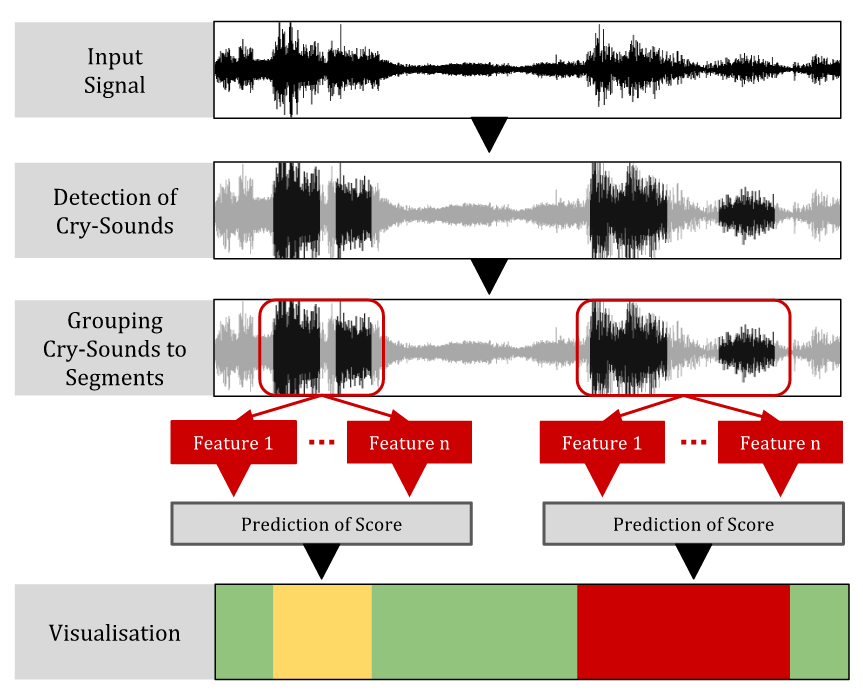
\includegraphics[width=0.75\textwidth]{bilder/konzept03.png}
	\caption{Überblick über die Verarbeitungs-Pipeline dieser Arbeit}
	\label{img:architecture-overview}
\end{figure}

Der erste Verarbeitungsschritt, die Erkennung der Schreigeräuschen, ist notwendig, damit für die Prognose des Scores für das Weinen auch nur solchen Informationen genutzt werden, die tatsächlich von einem Baby stammen, und nicht das Hintergrundrauschen. Würde man beispielsweise das Scoring für das Weinen hauptsächlich auf der Tonhöhe des Weinens ableiten und vorher nicht solche Geräusche verwerfen, die nicht von einem Baby stammen, würde diese mit in die Berechnung des Scores einfließen und das Ergebnis verfälschen. Diese Notwendigkeit wurde sowohl von Várallyay \cite{cry_thesis} als auch von Cohen et al. \cite{cohenCry} beschrieben. 


Der zweite Verarbeitungsschritt, die Segmentierung, ist notwendig, da wie in Kapitel \ref{sec:medicalFoundations} beschrieben der Schmerz-Score für einen längeren Beobachtungszeitraum bestimmt wird und in einem kontinuierlichen System sinnvolle Anfangs- und Endzeitpunkte für diese Beobachtungszeiträume gefunden werden müssen. Keine der in Kapitel \ref{sec:system_literature} vorgestellten Veröffentlichungen stellt ein Methode zur Gruppierung der Schreigeräusche vor, die für diese Arbeit übernommen werden könnte. Cohen et al. \cite{cohenCry} schlägt eine Feste Segmentlänge von 10 Sekunden vor. Es wurde sich gegen diesen Ansatz entschieden, da einige der in Kapitel \ref{sec:medicalFoundations} beschriebenen Pain-Scales längere Beobachtungszeiträume fordern. In der Promotion von Várallyay \cite{cry_thesis} war dieser Verarbeitungsschritt nicht notwendig, da die Analyse nicht kontinuierlich umgesetzt werden musste und die zu Analysierenden Segmente manuell geschnitten wurden. Pal et al. \cite{palEmotion} erwähnen keine Gruppierung von Schregeräuschen. Deshalb wurde in dieser Arbeit ein simpler Algorithmus zur Segmentierung entwickelt, welcher in Kapitel \ref{sec:segmenting} vorgestellt wird.

Die Berechnung von akustischen Eigenschaften des Weinens und der darauf folgenden Prongnose des Schmerz-Scores ist ein Verarbeitungschritt, der grundlegend in allen in Kapitel \ref{sec:system_literature} vorgestellten Veröffentlichungen angewendet wird. Je nach Ziel der Prognose werden unterschiedliche Eigenschaften und Klassifizierungs- oder Regressionsmethoden berechnet. 


\subsection{Automatisierte Visualisierung der Schmerzbewertung im multimodalen Verbund}



Dies würde der Visualisierung eines Schmerz-Score entsprechen, insofern es sich bei der verwendeten Schmerz-Scale allein um eine monomodale Scale handelt, die nur das Weinen in das Scoring mit einbezieht. In einem multimodalen System müssten vor der Visualisierung die Scores der anderen Schmerzindikatoren dem für das Weinen vergebenen Score aufaddiert werden. In diesem Fall wäre das Visualisierungskonzept ebenfalls anwendbar.